\subsection{Background Reduction and \ttbar Veto}
\label{subsec:bkg-reduction}

\hl{Rui wrote this - I need to rephrase!}

In order to suppress background, a pseudorapidity separation of $\deta < 1.5$ is required between the two Higgs candidates in the ggF channel. This cut is not used in the VBF channel as it reduces sensitivity to SM VBF \HH production. \Fig{\ref{fig:dEta-ggf}} shows the \deta distributions for ggF \HH signal and blinded data\footnote{By blinded data, we mean we do not show data events that fall in our 4b signal region as defined by \Eqn{\ref{eq:xhh}}.} in the ggF channel immediately after the pairing. It demonstrates that the data in the $(m_{H1}, m_{H2})$ plane, which is a good approximation of the background, tends to have higher values than those of the signal. Therefore, such a cut is applied to improve the signal purity.
It is worth mentioning that a cut on the Higgs candidate \pt was applied in the previous publication, but was found to not be as powerful in the recent resonant search~\cite{pT_Cut_and_Muon-in-jet_Correction}.
Therefore, it is dropped in this analysis.

\begin{figure}[b]
    \centering
    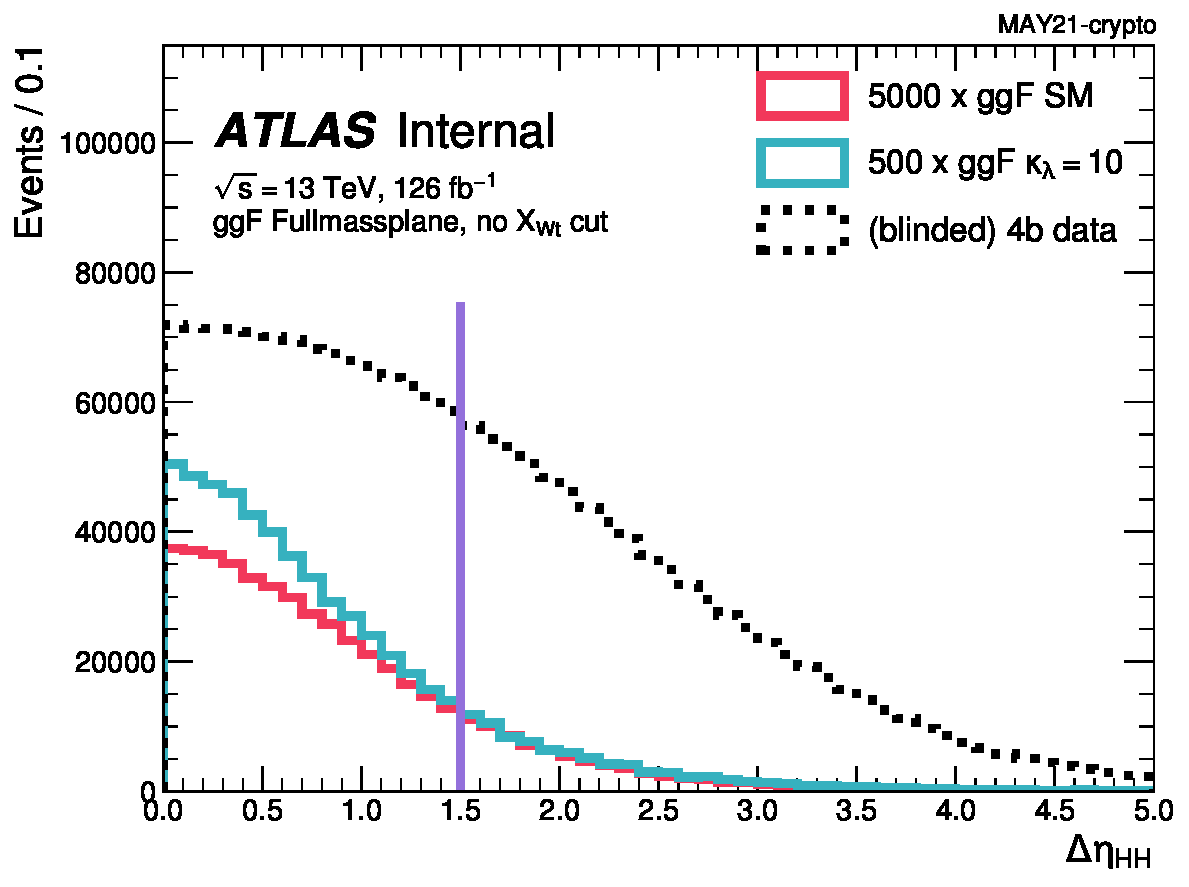
\includegraphics[width=0.5\textwidth]{figures/nr-int-note/selection/V3/dEta_hh_ggF_fullmassplane_all_4b_sm_k10.pdf}
    \caption{The \deta distribution for SM ggF \HH Monte Carlo simulation and blinded data in the ggF channel. The solid purple line indicates the \deta < 1.5 cut that is applied in the ggF selection. Events to the right of this line are discarded.}
    \label{fig:dEta-ggf}
\end{figure}

Additionally, a top veto is applied to suppress the background from hadronic top-quark decays.
This is applied by cutting on a discriminant, $\Xwt$, that is constructed to measure the compatibility of an event to contain a hadronically decaying top-quark.
To construct $\Xwt$, \PW candidates are formed from any pair of jets with $\pt > \SI{40}{\GeV}$ and $|\eta| < 2.5$, including those that were not selected for the Higgs candidates or for the VBF jets.
All possible \PW candidates are considered, and top candidates are built by pairing \PW candidates with any remaining \Pqb-jets that were selected for Higgs candidates.
The discriminant $\Xwt$ is constructed for each combination, expressed as:
\begin{equation}
    \Xwt = \sqrt{\left(\frac{m_{\PW} - \SI{80.4}{\GeV}}{0.1 \ m_{\PW}}\right)^{2} + \left(\frac{m_{\Pqt} - \SI{172.5}{\GeV}}{0.1 \ m_{\Pqt}}\right)^{2}}
    \label{eqn:xwt}
\end{equation}
Events are then vetoed if the minimum $\Xwt$ over all combinations is less than \num{1.5}.
\Fig{\ref{fig:Xwt}} shows the effectiveness of this cut at reducing the $t\bar{t}$ background while keeping a high efficiency for our signals.

\begin{figure}[ht]
	\centering
	\subfloat[4b ggF selection]{ %  with the ggF selection
	    	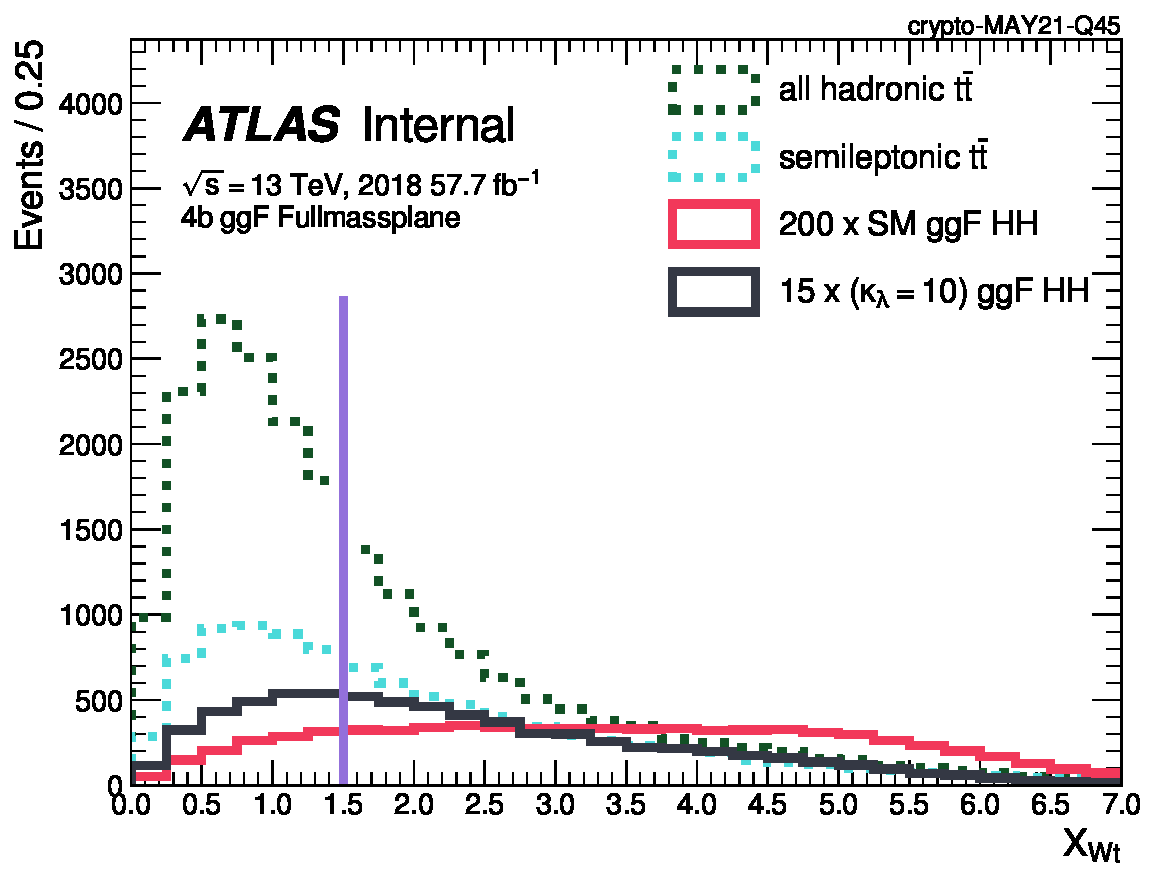
\includegraphics[width=0.44\textwidth]{figures/nr-int-note/selection/V4/X_wt_tag-ggf-4b-18}
		\label{fig:Xwt-ggf-4b}
	}
	\subfloat[4b VBF selection]{ % with the VBF selection
	    	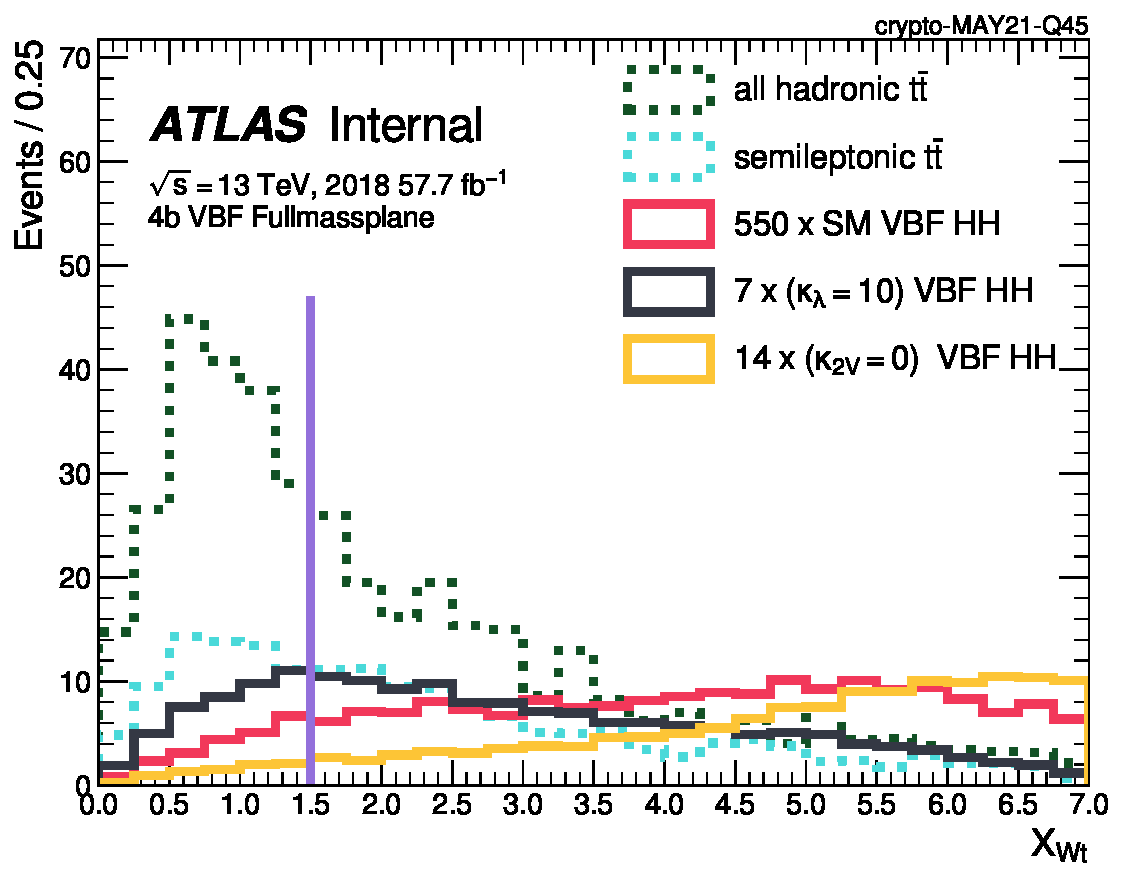
\includegraphics[width=0.44\textwidth]{figures/nr-int-note/selection/V4/X_wt_tag-vbf-4b-18}
 		\label{fig:Xwt-ggf-4b}
	}
	\caption{\Xwt distributions for our analysis categories in the 2018 dataset.
	The solid pink line indicates the $\Xwt$ > 1.5 cut applied to both the ggF and VBF channels.
	Event on the left of the line are discarded.}
	\label{fig:Xwt}
\end{figure}


We require the jet from Higgs candidates that is paired with the \PW candidate to be \textbf{\Pqb-tagged} while in the previous analyses there is no such a requirement.
%Although this requirement does not have any impact on the 4b events, it impacts 2b events, lowering the uncertainties on the background estimate\footnote{\href{https://indico.cern.ch/event/994939/contributions/4182687/}{https://indico.cern.ch/event/994939/contributions/4182687/}}.
% If I want to say this, I think I'll need to include the plots
